\documentclass{standalone}
\usepackage{tikz}
\usetikzlibrary{patterns, positioning}


\begin{document}
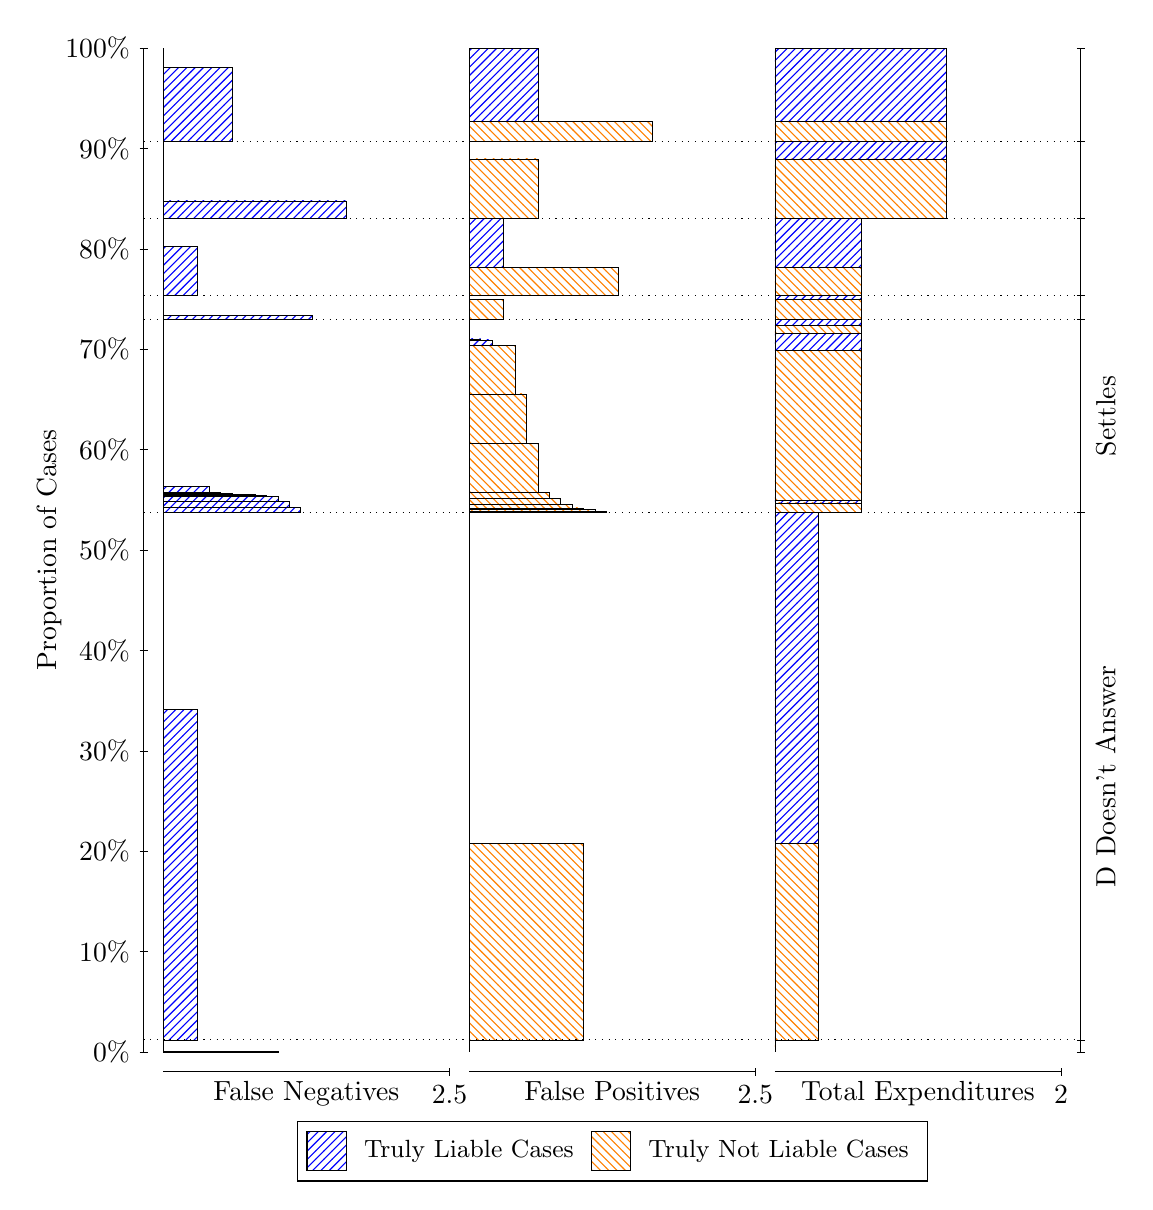
\begin{tikzpicture}
\draw[black, very thin] (1.5,1.75) -- (1.5,14.5);
\node[rotate=90, text=black, anchor=center] at (0.3, 8.125) {Proportion of Cases};
\draw[black, very thin] (1.45,1.75) -- (1.55,1.75);
\node[text=black, anchor=east] at (1.45, 1.75) {0\%};
\draw[black, very thin] (1.45,3.025) -- (1.55,3.025);
\node[text=black, anchor=east] at (1.45, 3.025) {10\%};
\draw[black, very thin] (1.45,4.3) -- (1.55,4.3);
\node[text=black, anchor=east] at (1.45, 4.3) {20\%};
\draw[black, very thin] (1.45,5.575) -- (1.55,5.575);
\node[text=black, anchor=east] at (1.45, 5.575) {30\%};
\draw[black, very thin] (1.45,6.85) -- (1.55,6.85);
\node[text=black, anchor=east] at (1.45, 6.85) {40\%};
\draw[black, very thin] (1.45,8.125) -- (1.55,8.125);
\node[text=black, anchor=east] at (1.45, 8.125) {50\%};
\draw[black, very thin] (1.45,9.4) -- (1.55,9.4);
\node[text=black, anchor=east] at (1.45, 9.4) {60\%};
\draw[black, very thin] (1.45,10.675) -- (1.55,10.675);
\node[text=black, anchor=east] at (1.45, 10.675) {70\%};
\draw[black, very thin] (1.45,11.95) -- (1.55,11.95);
\node[text=black, anchor=east] at (1.45, 11.95) {80\%};
\draw[black, very thin] (1.45,13.225) -- (1.55,13.225);
\node[text=black, anchor=east] at (1.45, 13.225) {90\%};
\draw[black, very thin] (1.45,14.5) -- (1.55,14.5);
\node[text=black, anchor=east] at (1.45, 14.5) {100\%};

\draw[black, very thin] (13.4,1.75) -- (13.4,14.5);
\draw[black, very thin] (13.35,1.75) -- (13.45,1.75);
\node[anchor=west] at (13.35, 1.75) {};
\draw[black, very thin] (13.35,1.9031) -- (13.45,1.9031);
\node[anchor=west] at (13.35, 1.9031) {};
\draw[black, very thin] (13.35,8.5998) -- (13.45,8.5998);
\node[anchor=west] at (13.35, 8.5998) {};
\draw[black, very thin] (13.35,11.054) -- (13.45,11.054);
\node[anchor=west] at (13.35, 11.054) {};
\draw[black, very thin] (13.35,11.359) -- (13.45,11.359);
\node[anchor=west] at (13.35, 11.359) {};
\draw[black, very thin] (13.35,12.336) -- (13.45,12.336);
\node[anchor=west] at (13.35, 12.336) {};
\draw[black, very thin] (13.35,13.315) -- (13.45,13.315);
\node[anchor=west] at (13.35, 13.315) {};
\draw[black, very thin] (13.35,14.5) -- (13.45,14.5);
\node[anchor=west] at (13.35, 14.5) {};

\draw[black, very thin, pattern color=blue, pattern=north east lines] (1.75,1.75) rectangle (3.2033,1.759);
\draw[black, very thin, pattern color=orange, pattern=north west lines] (1.75,1.759) rectangle (1.75,1.9031);
\draw[black, very thin, pattern color=blue, pattern=north east lines] (1.75,1.9031) rectangle (2.186,6.1047);
\draw[black, very thin, pattern color=orange, pattern=north west lines] (1.75,6.1047) rectangle (1.75,8.5998);
\draw[black, very thin, pattern color=blue, pattern=north east lines] (1.75,8.5998) rectangle (3.494,8.6693);
\draw[black, very thin, pattern color=blue, pattern=north east lines] (1.75,8.6693) rectangle (3.3487,8.7382);
\draw[black, very thin, pattern color=blue, pattern=north east lines] (1.75,8.7382) rectangle (3.2033,8.807);
\draw[black, very thin, pattern color=blue, pattern=north east lines] (1.75,8.807) rectangle (3.058,8.812);
\draw[black, very thin, pattern color=blue, pattern=north east lines] (1.75,8.812) rectangle (3.058,8.8164);
\draw[black, very thin, pattern color=blue, pattern=north east lines] (1.75,8.8164) rectangle (2.9127,8.8271);
\draw[black, very thin, pattern color=blue, pattern=north east lines] (1.75,8.8271) rectangle (2.7673,8.8328);
\draw[black, very thin, pattern color=blue, pattern=north east lines] (1.75,8.8328) rectangle (2.622,8.8465);
\draw[black, very thin, pattern color=blue, pattern=north east lines] (1.75,8.8465) rectangle (2.4767,8.8598);
\draw[black, very thin, pattern color=blue, pattern=north east lines] (1.75,8.8598) rectangle (2.3313,8.9307);
\draw[black, very thin, pattern color=orange, pattern=north west lines] (1.75,8.9307) rectangle (1.75,11.054);
\draw[black, very thin, pattern color=blue, pattern=north east lines] (1.75,11.054) rectangle (3.6393,11.105);
\draw[black, very thin, pattern color=orange, pattern=north west lines] (1.75,11.105) rectangle (1.75,11.359);
\draw[black, very thin, pattern color=blue, pattern=north east lines] (1.75,11.359) rectangle (2.186,11.983);
\draw[black, very thin, pattern color=orange, pattern=north west lines] (1.75,11.983) rectangle (1.75,12.336);
\draw[black, very thin, pattern color=blue, pattern=north east lines] (1.75,12.336) rectangle (4.0753,12.558);
\draw[black, very thin, pattern color=orange, pattern=north west lines] (1.75,12.558) rectangle (1.75,13.315);
\draw[black, very thin, pattern color=blue, pattern=north east lines] (1.75,13.315) rectangle (2.622,14.25);
\draw[black, very thin, pattern color=orange, pattern=north west lines] (1.75,14.25) rectangle (1.75,14.5);
\draw[black, very thin, pattern color=orange, pattern=north west lines] (5.6333,1.75) rectangle (5.6333,1.8941);
\draw[black, very thin, pattern color=blue, pattern=north east lines] (5.6333,1.8941) rectangle (5.6333,1.9031);
\draw[black, very thin, pattern color=orange, pattern=north west lines] (5.6333,1.9031) rectangle (7.0867,4.3982);
\draw[black, very thin, pattern color=blue, pattern=north east lines] (5.6333,4.3982) rectangle (5.6333,8.5998);
\draw[black, very thin, pattern color=orange, pattern=north west lines] (5.6333,8.5998) rectangle (7.3773,8.6196);
\draw[black, very thin, pattern color=orange, pattern=north west lines] (5.6333,8.6196) rectangle (7.232,8.6375);
\draw[black, very thin, pattern color=orange, pattern=north west lines] (5.6333,8.6375) rectangle (7.0867,8.6587);
\draw[black, very thin, pattern color=orange, pattern=north west lines] (5.6333,8.6587) rectangle (6.9413,8.702);
\draw[black, very thin, pattern color=orange, pattern=north west lines] (5.6333,8.702) rectangle (6.796,8.7851);
\draw[black, very thin, pattern color=orange, pattern=north west lines] (5.6333,8.7851) rectangle (6.6507,8.8603);
\draw[black, very thin, pattern color=orange, pattern=north west lines] (5.6333,8.8603) rectangle (6.5053,9.483);
\draw[black, very thin, pattern color=orange, pattern=north west lines] (5.6333,9.483) rectangle (6.36,10.107);
\draw[black, very thin, pattern color=orange, pattern=north west lines] (5.6333,10.107) rectangle (6.2147,10.723);
\draw[black, very thin, pattern color=blue, pattern=north east lines] (5.6333,10.723) rectangle (5.924,10.794);
\draw[black, very thin, pattern color=blue, pattern=north east lines] (5.6333,10.794) rectangle (5.7787,10.807);
\draw[black, very thin, pattern color=blue, pattern=north east lines] (5.6333,10.807) rectangle (5.6333,11.054);
\draw[black, very thin, pattern color=orange, pattern=north west lines] (5.6333,11.054) rectangle (6.0693,11.308);
\draw[black, very thin, pattern color=blue, pattern=north east lines] (5.6333,11.308) rectangle (5.6333,11.359);
\draw[black, very thin, pattern color=orange, pattern=north west lines] (5.6333,11.359) rectangle (7.5227,11.712);
\draw[black, very thin, pattern color=blue, pattern=north east lines] (5.6333,11.712) rectangle (6.0693,12.336);
\draw[black, very thin, pattern color=orange, pattern=north west lines] (5.6333,12.336) rectangle (6.5053,13.092);
\draw[black, very thin, pattern color=blue, pattern=north east lines] (5.6333,13.092) rectangle (5.6333,13.315);
\draw[black, very thin, pattern color=orange, pattern=north west lines] (5.6333,13.315) rectangle (7.9587,13.564);
\draw[black, very thin, pattern color=blue, pattern=north east lines] (5.6333,13.564) rectangle (6.5053,14.5);
\draw[black, very thin, pattern color=orange, pattern=north west lines] (9.5167,1.75) rectangle (9.5167,1.8941);
\draw[black, very thin, pattern color=blue, pattern=north east lines] (9.5167,1.8941) rectangle (9.5167,1.9031);
\draw[black, very thin, pattern color=orange, pattern=north west lines] (9.5167,1.9031) rectangle (10.062,4.3982);
\draw[black, very thin, pattern color=blue, pattern=north east lines] (9.5167,4.3982) rectangle (10.062,8.5998);
\draw[black, very thin, pattern color=orange, pattern=north west lines] (9.5167,8.5998) rectangle (10.607,8.7221);
\draw[black, very thin, pattern color=blue, pattern=north east lines] (9.5167,8.7221) rectangle (10.607,8.7597);
\draw[black, very thin, pattern color=orange, pattern=north west lines] (9.5167,8.7597) rectangle (10.607,10.662);
\draw[black, very thin, pattern color=blue, pattern=north east lines] (9.5167,10.662) rectangle (10.607,10.874);
\draw[black, very thin, pattern color=orange, pattern=north west lines] (9.5167,10.874) rectangle (10.607,10.973);
\draw[black, very thin, pattern color=blue, pattern=north east lines] (9.5167,10.973) rectangle (10.607,11.054);
\draw[black, very thin, pattern color=orange, pattern=north west lines] (9.5167,11.054) rectangle (10.607,11.308);
\draw[black, very thin, pattern color=blue, pattern=north east lines] (9.5167,11.308) rectangle (10.607,11.359);
\draw[black, very thin, pattern color=orange, pattern=north west lines] (9.5167,11.359) rectangle (10.607,11.712);
\draw[black, very thin, pattern color=blue, pattern=north east lines] (9.5167,11.712) rectangle (10.607,12.336);
\draw[black, very thin, pattern color=orange, pattern=north west lines] (9.5167,12.336) rectangle (11.697,13.092);
\draw[black, very thin, pattern color=blue, pattern=north east lines] (9.5167,13.092) rectangle (11.697,13.315);
\draw[black, very thin, pattern color=orange, pattern=north west lines] (9.5167,13.315) rectangle (11.697,13.564);
\draw[black, very thin, pattern color=blue, pattern=north east lines] (9.5167,13.564) rectangle (11.697,14.5);
\draw[black, dotted] (1.5,1.9031) -- (13.4,1.9031);
\draw[black, dotted] (1.5,8.5998) -- (13.4,8.5998);
\draw[black, dotted] (1.5,11.054) -- (13.4,11.054);
\draw[black, dotted] (1.5,11.359) -- (13.4,11.359);
\draw[black, dotted] (1.5,12.336) -- (13.4,12.336);
\draw[black, dotted] (1.5,13.315) -- (13.4,13.315);
\draw[black, very thin] (1.75,1.5) -- (5.3833,1.5);
\node[text=black, anchor=north] at (3.5667, 1.5) {False Negatives};
\draw[black, very thin] (5.3833,1.45) -- (5.3833,1.55);
\node[text=black, anchor=north] at (5.3833, 1.45) {2.5};

\draw[black, very thin] (5.6333,1.5) -- (9.2667,1.5);
\node[text=black, anchor=north] at (7.45, 1.5) {False Positives};
\draw[black, very thin] (9.2667,1.45) -- (9.2667,1.55);
\node[text=black, anchor=north] at (9.2667, 1.45) {2.5};

\draw[black, very thin] (9.5167,1.5) -- (13.15,1.5);
\node[text=black, anchor=north] at (11.333, 1.5) {Total Expenditures};
\draw[black, very thin] (13.15,1.45) -- (13.15,1.55);
\node[text=black, anchor=north] at (13.15, 1.45) {2};


\node[text=black, centered, rotate=90] at (13.72, 5.2515) {D Doesn't Answer};
\node[text=black, centered, rotate=90] at (13.72, 9.8267) {Settles};





\draw (7.449999999999999,1.5) node[draw=none] (baseCoordinate) {};
\begin{scope}[align=center]
        \matrix[scale=0.5, draw=black, below=0.5cm of baseCoordinate, nodes={draw}, column sep=0.1cm]{
            \node[rectangle, draw, minimum width=0.5cm, minimum height=0.5cm, pattern color=blue, pattern=north east lines] {}; &
            \node[draw=none, font=\small, text=black] (B) {Truly Liable Cases}; &
            \node[rectangle, draw, minimum width=0.5cm, minimum height=0.5cm, pattern color=orange, pattern=north west lines] {}; &
            \node[draw=none, font=\small, text=black] (B) {Truly Not Liable Cases}; \\
            };
\end{scope}

\end{tikzpicture}
\end{document}